\section{Introduction of 7 Mental Disorders}
\label{apd:dis_intro}
Here, we briefly introduce 7 mental disorders studied in our paper, listing their typical manifestations summarized from DSM-5 in Table \ref{tab:disease_intro} for better understanding of these mental disorders.

\begin{table}[th]
    \small
    \centering
    \begin{tabular}{m{2.2cm}|m{4cm}}
        \hline
        Disease          & Typical Symptoms \\
        \hline
        ADHD             & inattention; hyperactivity and impulsivity.         \\
        \hline
        Anxiety          &  excessive fear and worry; panic attacks; anxious mood.       \\
        \hline
        Bipolar Disorder & drastic shift in mood and energy; experience periods of mania and depression.        \\
        \hline
        Depression       &  depressed mood; loss of pleasure or interest; poor concentration; guilty feelings; suicidal ideas.      \\
        \hline
        Eating Disorder  &  intense fear of gaining weight; binge and purge; rumination; weight and appetite change.        \\
        \hline
        OCD              & obsession; compulsion.         \\
        \hline
        PTSD             &  often develops after a shocking, dangerous event; flashbacks; bad dreams.        \\
        \hline
    \end{tabular}
    \caption{7 mental disorders detected in our work with their typical symptoms.}
    \label{tab:disease_intro}
\end{table}

\section{Detailed Data Statistics}
\label{apd:stats}

For the multiple MDD datasets (Section \ref{sec:mdd_dataset}), we show the number of users suffering from each disease in Table \ref{tab:disease_detect_count}. The distribution of the 7 diseases are similar to SMHD \citep{cohan2018smhd}, and the  training/validation/testing set is 8:1:1. 
\begin{table}[th]
    \small
    \centering
    \begin{tabular}{l|cc}
    \hline
    Disease          & \# Users (Reddit) & \# Users (Twitter)\\
    \hline
    Depression       & 3105 & 1448         \\
    Anxiety          & 2239 & 933        \\
    % Autism           & 716         \\
    ADHD             & 2374 & 1370        \\
    Bipolar Disorder & 1366 & 2011        \\
    OCD              & 753  & 368        \\
    PTSD             & 391  & 588        \\
    % Schizophrenia    & 345          \\
    Eating Disorder  & 138  & 0        \\
    \hline
    \end{tabular}
    \caption{Number of users suffering from each disease in the multiple MDD datasets (Reddit and Twitter).}
    \label{tab:disease_detect_count}
\end{table}

In addition, the users in these two datasets can suffer from multiple mental disorders simultaneously. So we also provide the distribution of the number of diseases on a single user in Table \ref{tab:dis_num_distribution}. The statistic shows that 57\% users suffer from more than one mental disorders in the Reddit dataset, and PsyEx can achieve superior performance for its specific design targeting these comorbidity scenarios.
\begin{table}[th]
    \small
    \centering
    \begin{tabular}{c|cc}
    \hline
    \# Disease          & \# Users (Reddit) & \# Users (Twitter)\\
    \hline
    1   & 2326 & 2842         \\
    2   & 1738 & 1716        \\
    3   & 931  & 134       \\
    4   & 407  & 8       \\
    5   & 152  & 1        \\
    6   & 51   & 0       \\
    7   & 14   & 0  \\
    \hline
    \end{tabular}
    \caption{Distribution of a user's disease counts. For example, there are 1738 users suffering from two mental diseases in the Reddit dataset.}
    \label{tab:dis_num_distribution}
\end{table}

\begin{table*}[th]
    \centering
      \small
    \begin{tabular}{l|ccccccc|c}
    \hline
    Model &  Depression &Anxiety &ADHD &  Bipolar & OCD & PTSD &  Eating & Avg. F1 \\ 
    \hline
    Two-Stream PsyEx &  87.89&	\textbf{89.84}&	84.4&	\textbf{91.58}&	\textbf{81.69}&	\textbf{81.69}&	85.71 & \textbf{86.12}      \\
    ~~~~ w/o symp-stream & \textbf{88.12}&	89.09&	\textbf{84.55}&	89.33&	76.71&	81.58&	83.33 & 84.67 \\
    ~~~~ w/o multi-attn & 87.64&	88.64&	82.84&	89.7&	76.39&	79.49&	81.08 & 83.68       \\
    ~~~~ w/o multi-task & 87.69&	88.89&	84.21&	91.16&	75&	84.21&	\textbf{86.67} & 85.40     \\
    \hline
    \end{tabular}
    \caption{Ablation tests for the design choices of PsyEx, reporting F1 score of each disease (detailed results of Table \ref{tab:ablation}).}
    \label{tab:mdd_by_disease}
\end{table*}

\begin{table*}[th]
    \centering
    \small
    \begin{tabular}{l|ccccccc|c}
    \hline
    Screen method &  Depression &Anxiety &ADHD &  Bipolar & OCD & PTSD &  Eating & Avg. F1 \\ 
    \hline
    Symptom-based (PsyEx) &  \textbf{87.89}&	\textbf{89.84}&	\textbf{84.4}&	\textbf{91.58}&	\textbf{81.69}&	\textbf{81.69}&	\textbf{85.71} & \textbf{86.12}      \\
    Similarity & 86.84	&87.7	&83.03	&87.84&	78.26&	77.14&	76.47 & 82.47 \\
    K-Means & 79.34	&81.15	&68.66	&82.0&	70.34&	73.42&	68.42 & 74.76\\
    Last & 69.27&	67.89	&55.31	&67.6&	45.8	&46.15	&45.16 & 56.74    \\
    \hline
    \end{tabular}
    \caption{Ablation tests for different risky post screening methods, reporting F1 score of each disease (detailed results of Table \ref{tab:ablation_screen})}
    \label{tab:screen_by_disease}
\end{table*}

\section{Detailed Experimental Settings of Baselines}
\label{apd:settings}

% For all models, we empirically set hyperparameters following existing implementations and previous works without fine-tuning them for optimized performance. 
For the CNN backbone of \textit{BERT} and \textit{Symp} method, the model structure is the same as that of \citet{nguyen2022improving}. We train both model with batch size=64, but we set the learning rate as 0.01 when using symptom features, and as 0.003 when using BERT embedding. The \textit{HAN-GRU} model is trained with batch size=32 and learning rate=0.0001. The posting list will be truncated to preserve the earliest 256 posts at most. The average posting number of users in the dataset is 115.2, so 256 is safe enough to preserve almost all the posts of a user. 

In the ablation test of different risky post screening methods, the sentence BERT model we utilized for \textit{Similarity} and \textit{K-Means} is \texttt{paraphrase-MiniLM-L6-v2}. What's more, the \textit{Similarity} \cite{zhang2022psychiatric} method extracts key posts according to the cosine similarity between post and mental disease descriptions, which are the description of 38 symptoms (see Table \ref{tab:symp_id}) manually summarized from DSM-5. 

Further, to infer the symptoms mentioned in the posts, we perform some pre-processing steps. First, we use \textit{blingfire}\footnote{\url{https://github.com/microsoft/BlingFire}} to split a post into sentences. Then, we use regular expressions to filter out the hyperlink format like ``[anchor text] (web url)'' and preserve the anchor text. Finally, we remove sentences like ``[removed]''. 
\subsection{ChatGPT baseline}
Due to the input length limitation of ChatGPT, we utilize the screening method described in \secref{sec:symp_screen}, which selects 16 posts from the user history instead of using all of them.

To maximize the effectiveness of ChatGPT, we made substantial efforts in prompt engineering. Through this process, we observed that directly requesting prediction results yielded unsatisfactory performance in binary setting. To address this, we introduced the requirement for ChatGPT to provide explanations alongside its predictions, leading to a significant improvement in accuracy, especially eating disorder (See \tabref{tab:chatgpt}). We also attempted to include explanation instructions in a multi-label setting; however, the outcome was even worse than without explanations. This suggests that there is still a long way to go in effectively utilizing ChatGPT for this task, and we hope to address this in the future work.
\begin{table*}[th]
    \small
    \centering
    \begin{tabular}{l|ccccccc|c}
    \hline
    Method & Depression & Anxiety & ADHD & Bipolar & OCD & PTSD & Eating &  Avg. F1 \\ 
    \hline
     direct & 66.92&70.16&	59.36&	67.95&	39.22&	53.13&	8.7&	52.21  \\
    \hline
     explanation & 70.12	&73.09	&64.08	&67.12	&52.98	&67.61	&29.73	&60.68 \\ 
    \hline
    \end{tabular}
    \caption{Mental disease detection results across 7 diseases utilizing ChatGPT in binary setting}
    \label{tab:chatgpt}
\end{table*}



We present the final prompts for both binary and multi-label settings below.
\paragraph{Binary setting} 
\begin{prompt}
    Please predict whether the user has mental disorders, such as {DISEASE}, from the clues showed in his/her posts on reddit. Your answer should be a single 'yes' or 'no', followed by an explanation of the predicted result.
\end{prompt}
\paragraph{Multi-label setting}
\begin{prompt}
Please predict the user's mental disorders according to his/her posts on reddit. The mental disoders should be chosen from: `depression', `anxiety', `bipolar', `eating disorder', `ADHD', `PTSD', `OCD'. The user can have multiple disorders, or have no disorder. Your answer format should be:  `mental disorders: \{MENTAL DISORDERS\}'.
\end{prompt}


\section{Detailed Ablation Results}
\label{apd:abl_results}
% \MY{Can you organise the table layout? Current Appendix looks messy}
We show the detailed results of ablation tests in Table \ref{tab:mdd_by_disease} and Table \ref{tab:screen_by_disease}.
Without symptom stream (i.e., w/o symp-stream) or disease-specific attention layer (i.e., w/o multi-attn), the F1 score on nearly all the diseases dropped, especially the rarer diseases like eating disorder and OCD. What's more, we can notice a significant drop in the performance without symptom-based risky post screening in all the diseases, suggesting the importance of a precise screening method to filter out the noisy data.

\subsection{Impact of the Number of Selected Posts}
\label{apd:post_num}
Here we study the impact of the number of posts selected in risky posts screening (see Figure~\ref{fig:post_num}). We can observe that 16 posts have the best performance for nearly all the diseases. To find out the reason, we calculate the average symptom probability of the selected $K$ posts sorted by its highest symptom probability, which is 0.25 for the posts ranked 16, meaning that 16 posts is enough to include most of the symptomatic posts and adding more posts can easily introduce some noisy data.

\begin{figure}[th]
    \centering
    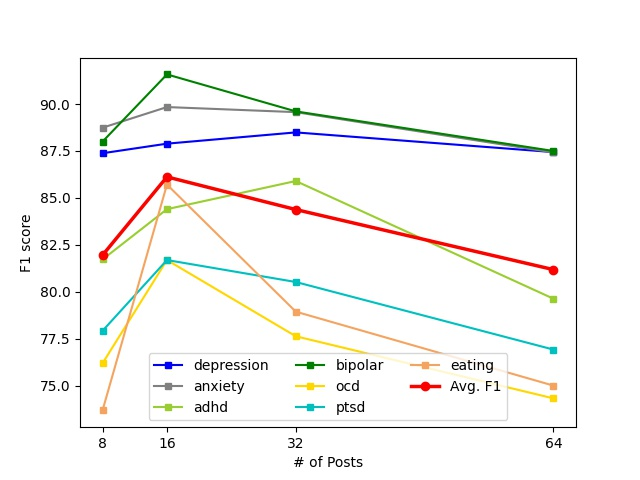
\includegraphics[width=\linewidth]{figures/post_num_impact.jpg}
    \caption{Impact of the number of selected posts on each disease and the mean F1.}
    \label{fig:post_num}
\end{figure}

\section{Psychiatric Symptoms}
\label{apd:symps}
We use serial numbers to represent symptoms in Figure \ref{fig:symp_stream_score} and Figure \ref{fig:symp_contribution}, so we provide the corresponding symptom names in Table \ref{tab:symp_id} for reference. 

These symptoms are defined in the symptom identification dataset proposed by \citet{Zhang2022SymptomIF}. This dataset contains 8,554 sentences extracted from the Reddit corpus. All the sentences are annotated with symptoms that can be identified from the sentence. The average Fleiss’s $\kappa$ for all the 38 symptoms is 0.7708.
\begin{table}[th]
    \small
    \centering
    \begin{tabular}{m{0.4cm}m{6cm}}
    \hline
    id & Symptom  \\
    \hline
    1&Anxious Mood 	\\
    2&Autonomic symptoms	\\
    3&Cardiovascular symptoms		\\
    4&Catatonic behavior\\
    5&Decreased energy tiredness fatigue	\\
    6&Depressed Mood\\
    7&Gastrointestinal symptoms	\\
    8&Genitourinary symptoms	\\
    9&Hyperactivity agitation	\\
    10&Impulsivity		\\
    11&Inattention	\\
    12&Indecisiveness	\\
    13&Respiratory symptoms\\
    14&Suicidal ideas	\\
    15&Worthlessness and guilty	\\
    16&Avoidance of stimuli	\\
    17&Compensatory behaviors to prevent weight gain	\\
    18&Compulsions		\\
    19&Diminished emotional expression		\\
    20&Do things easily get painful consequences	\\
    21&Drastic shift in mood and energy	\\
    22&Fear about social situations	\\
    23&Fear of gaining weight	\\
    24&Fears of being negatively evaluated	\\
    25&Flight of ideas	\\
    26&Intrusion symptoms	\\
    27&Loss of interest or motivation	\\
    28&More talkative\\
    29&Obsession	\\
    30&Panic fear	\\
    31&Pessimism	\\
    32&Poor memory	\\
    33&Sleep disturbance	\\
    34&Somatic muscle		\\
    35&Somatic symptoms others		\\
    36&Somatic symptoms sensory	\\
    37&Weight and appetite change	\\
    38&Anger Irritability	\\
    \hline
    \end{tabular}
    \caption{Id and its corresponding symptoms}
    \label{tab:symp_id}
\end{table}
% \begin{table*}[t]
%     \centering
%     \resizebox{\textwidth}{15mm}{
%     \begin{tabular}{m{1.5cm}|m{0.08cm}m{0.08cm}m{0.08cm}m{0.08cm}m{0.08cm}m{0.08cm}m{0.08cm}m{0.08cm}m{0.08cm}m{0.08cm}m{0.08cm}m{0.08cm}m{0.08cm}m{0.08cm}m{0.08cm}m{0.08cm}m{0.08cm}m{0.08cm}m{0.08cm}m{0.08cm}m{0.08cm}m{0.08cm}m{0.08cm}m{0.08cm}m{0.08cm}m{0.08cm}m{0.08cm}m{0.08cm}m{0.08cm}m{0.08cm}m{0.08cm}m{0.08cm}m{0.08cm}m{0.08cm}m{0.08cm}m{0.08cm}m{0.08cm}m{0.08cm}}
%     \hline
%     Disease          & 1 & 2 & 3 & 4 & 5 & 6 & 7 & 8 & 9 & 10 & 11 & 12 & 13 & 14 & 15 & 16 & 17 & 18 & 19 & 20 & 21 & 22 & 23 & 24 & 25 & 26 & 27 & 28 & 29 & 30 & 31 & 32 & 33 & 34 & 35 & 36 & 37 & 38 \\
%     \hline
%     ADHD & & & & & & & & & \checkmark &\checkmark &\checkmark & & & & & & & & & & & & & & & & &\checkmark & & & & & & & & & & \\
%     \hline
%     Anxiety &\checkmark &\checkmark &\checkmark & &\checkmark &\checkmark &\checkmark &\checkmark &\checkmark & &\checkmark & &\checkmark & & & & & & & & &\checkmark & &\checkmark & & & & & &\checkmark & &\checkmark &\checkmark &\checkmark &\checkmark &\checkmark & &\checkmark \\
%     \hline
%     Bipolar & & & & &\checkmark &\checkmark & & &\checkmark & &\checkmark & & &\checkmark &\checkmark & & & & &\checkmark &\checkmark & & & &\checkmark & &\checkmark &\checkmark & & & & &\checkmark & & & &\checkmark &\checkmark \\
%     \hline
%     Depression & & & & &\checkmark &\checkmark & &\checkmark &\checkmark & &\checkmark &\checkmark & &\checkmark &\checkmark & & & & & & & & & & & &\checkmark & & & &\checkmark &\checkmark &\checkmark & & & &\checkmark &\checkmark \\
%     \hline
%     Eating & & & & & &\checkmark & &\checkmark & & & & & & &\checkmark & &\checkmark & &\checkmark & & & &\checkmark &\checkmark & & &\checkmark & &\checkmark & & & &\checkmark & & & &\checkmark &\checkmark \\
%     \hline
%     OCD &\checkmark & & & & &\checkmark & & & & & & & & & & & &\checkmark & & & & & & & & & & &\checkmark & & & & & & & & & \\
%     \hline
%     PTSD &\checkmark &\checkmark & &\checkmark & & & & & & &\checkmark & & & &\checkmark &\checkmark & & &\checkmark &\checkmark & & & & & &\checkmark &\checkmark & & & &\checkmark &\checkmark &\checkmark & & & & &\checkmark \\
%     \hline
%     \end{tabular}}
%     \caption{Symptoms of 7 mental disorders summarized from DSM-5.}
%     \label{tab:symp_of_dsm5}
% \end{table*}

% \section{Detailed Symptom Contribution Results}
% \label{apd:symp_contribution}
% We use serial numbers to represent symptoms in Figure \ref{fig:symp_contribution}, and provide the corresponding symptom names in Table \ref{tab:symp_id} for reference. 


% For comparison, we demonstrate the symptom-disease connection extracted from the diagnosis criteria DSM-5 in Table \ref{tab:symp_of_dsm5}. 
